% Chapter Template

\chapter{Diagrammatic notation} % Main chapter title

\label{Chapter3} % Change X to a consecutive number; for referencing this chapter elsewhere, use \ref{ChapterX}

\lhead{Chapter 3. \emph{Diagrammatic notation}} % Change X to a consecutive number; this is for the header on each page - perhaps a shortened title

%----------------------------------------------------------------------------------------
%	Diagrammatic notation
%----------------------------------------------------------------------------------------

\section{Diagrammatic notation - background}

While Second Quantization provides us with the foundation for working out expressions within the various many body methods, it may prove cumbersome to derive comprehensive equations such as the Coupled Cluster equations using only second quantized operators and Wick's generalized theorem. To this end, the \emph{diagrammatic notation}, originally introduced into quantum electro dynamics by Richard Feynman in 1959 \cite[p.1]{ShavittBartlett2009}, will simplify calculations considerably. In addition, the diagrams will allow us to easily identify features of terms in the equations such as which terms vanish or should be naturally grouped together. \cite{ShavittBartlett2009}

\section{The Slater Determinant}

Due to their origin in quantum field theory, the diagrams will actually express a time ordered sequence of operators where time evolve in the upwards direction. This might seem strange when applied to the time independent Schrödinger equation, but we shall only interpret the time axis as the sequence in which the different operators are applied. A starting point for the calculations will be the Fermi vacuum, expressed simply by a blank space. As we have already shown \ref{}, normal ordering of the hamiltonian with respect to the Fermi vacuum will allow us mainly focus on excited SDs. These kind of SDs may be expressed simply by vertical lines, assigned either upwards- or downwards arrows to indicate particle or holes, respectively, as in \ref{fig:diag_psi_ai} or \ref{fig:diag_psi_aibj}. 

\begin{figure}[p]
    \centering
    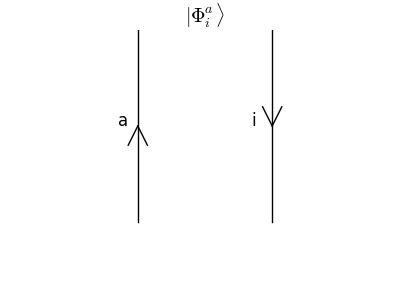
\includegraphics[width=0.5\textwidth]{diag_psi_ai}
    \caption{A slater determinant with one hole and one particle state.}
    \label{fig:diag_psi_ai}
\end{figure}

\begin{figure}[p]
    \centering
    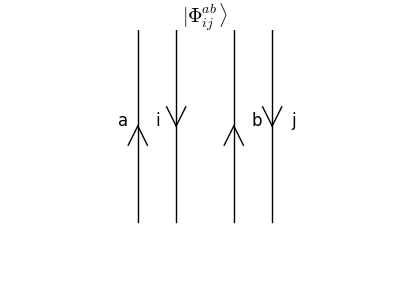
\includegraphics[width=0.5\textwidth]{diag_psi_aibj}
    \caption{A slater determinant with two holes and two particle states.}
    \label{fig:diag_psi_aibj}
\end{figure}

\section{Operators}

We will use horizontal dashed lines to represent operators such as terms in the normal ordered hamiltonian. While the one body operator will have two lines entering and/or leaving, the two body operator will have four lines entering and/or leaving. The lines entering from below represents the annihilation of pseudo particles, while lines exiting above represents creation of pseudo particles. Following this logic, we list the normal ordered one body operator (\ref{eqn:onebody_N}) and the normal ordered two body operator (\ref{fig:onebody}) diagrammatically in the figures \ref{fig:onebody}, \ref{fig:twobody1} and \ref{fig:twobody2}.

\begin{figure}[p]
    \centering
    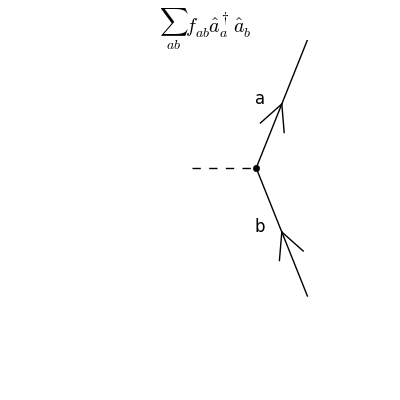
\includegraphics[width=0.4\textwidth]{onebody1}
    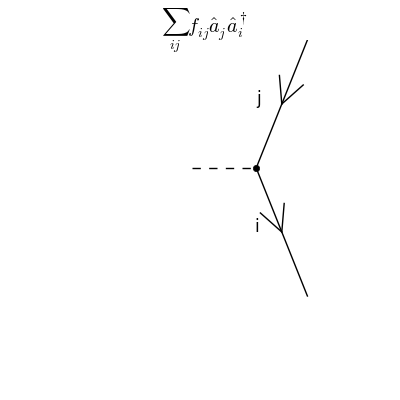
\includegraphics[width=0.4\textwidth]{onebody2}
    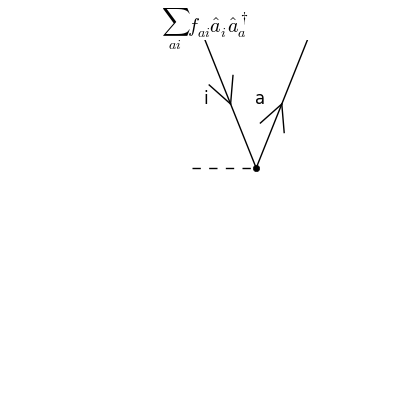
\includegraphics[width=0.4\textwidth]{onebody3}
    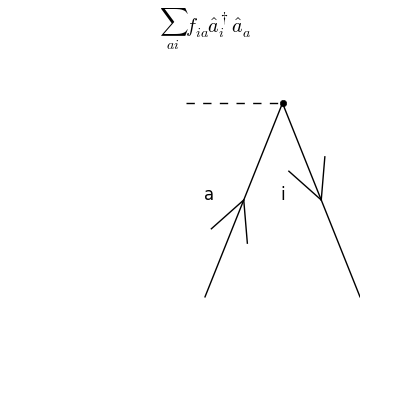
\includegraphics[width=0.4\textwidth]{onebody4}
    \caption{A normal ordered one body operator}
    \label{fig:onebody}
\end{figure}

\begin{figure}[p]
    \centering
    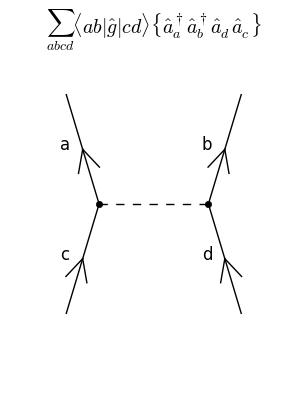
\includegraphics[width=0.4\textwidth]{twobody1}
    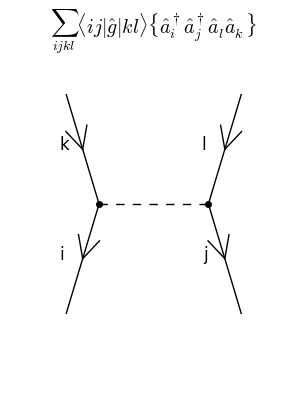
\includegraphics[width=0.4\textwidth]{twobody2}
    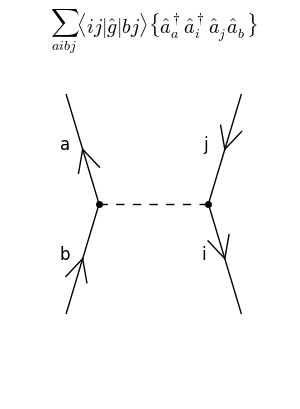
\includegraphics[width=0.4\textwidth]{twobody3}
    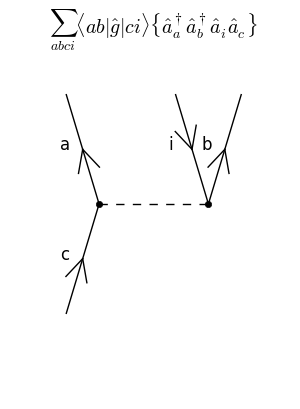
\includegraphics[width=0.4\textwidth]{twobody4}
    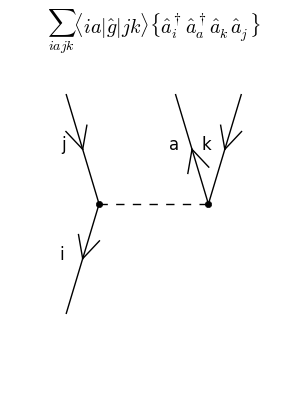
\includegraphics[width=0.4\textwidth]{twobody5}
    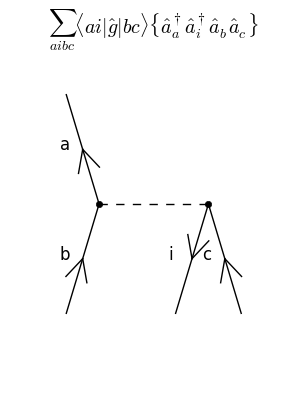
\includegraphics[width=0.4\textwidth]{twobody6}
    \caption{A normal ordered two body operator}
    \label{fig:twobody1}
\end{figure}

\begin{figure}[p]
    \centering
    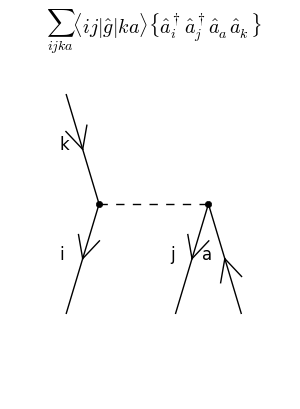
\includegraphics[width=0.4\textwidth]{twobody7}
    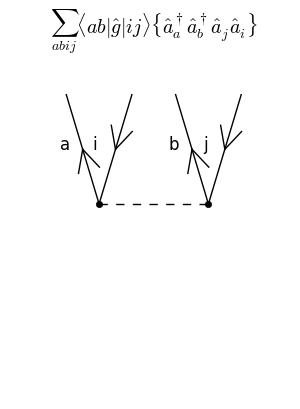
\includegraphics[width=0.4\textwidth]{twobody8}
    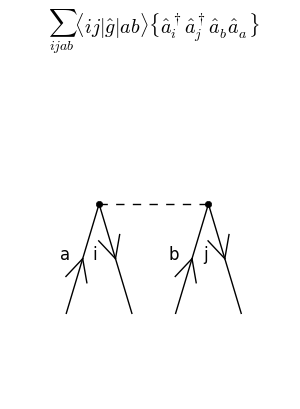
\includegraphics[width=0.4\textwidth]{twobody9}
    \caption{A normal ordered two body operator (continued)}
    \label{fig:twobody2}
\end{figure}

\section{Contractions}

The diagrams will enable us to represent contractions in a straight forward manner, by connecting lines from SDs to operators or between operators. For example, we may consider the contraction of a singly excited SD with a term in the normal ordered one body operator:

\begin{equation}
( \sum_{bc} f_{bc} \{  \Cr{b} \An{c} \}) \vert \Phi_i^a \rangle = ( \sum_{bc} f_{bc} \{ \Cr{b} \An{c} \})\{ \Cr{a} \An{i} \} \vert \Phi_0 \rangle = \sum_{bc} f_{bc} \delta_{ac}  \vert \Phi_i^b \rangle 
\label{eqn:onebody_N1}
\end{equation}

Where the contraction occurs between the indices in the Kronecker delta. The equivalent diagrammatic contraction is performed in ref{fig:contraction}

\begin{figure}[p]
    \centering
    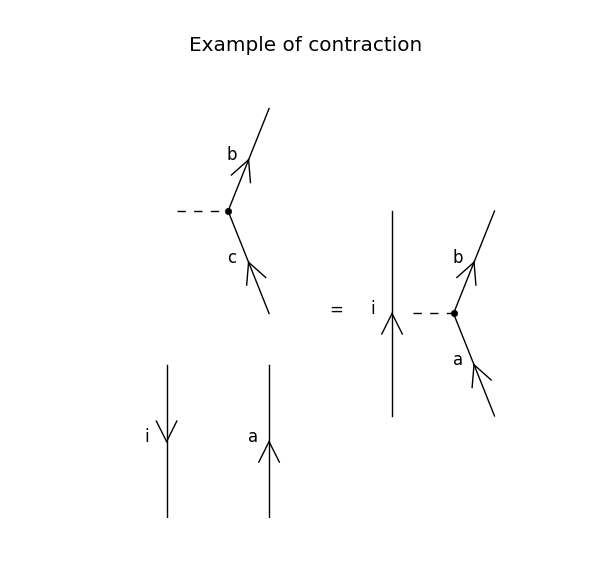
\includegraphics[width=0.7\textwidth]{contraction}
    \caption{A contraction of a one body operator and a singly excited Slater Determinant.}
    \label{fig:contraction}
\end{figure}

The diagrams resulting from this process may in turn be interpreted back into mathematical expressions that we may use in implementations of the various many body methods. 

\section{Interpreting diagrams}

The various many body methods which will be introduced in the upcoming chapters rely on operator expressions and contractions. The basic idea of using diagrams to derive such expressions may be outlined as follows. For a given method we shall see that the contracted expressions that needs evaluation to obtain the correlation energy may be visually represented by a set of diagrams. The situation before this contractions may also be visually represented by combinations of such uncontracted vertices as shown in figures \ref{fig:twobody1, fig:twobody2, fig:onebody1} (and so on). By defining consistent rules for how the contracted diagrams are obtained from the uncontracted vertices, we may skip the mathematical contraction altogether, derive the various resulting terms, and interpret them back into mathematical expressions by rules that ensure that all factors and distinct features of the expressions are preserved.

Luckily, such consistent rules is present in the literature \cite{ShavittBartlett2009} for many of the methods we discuss in the upcoming chapter.